% Figure: Cerebral Hypoperfusion in ME/CFS
% Reduced blood flow causes brain energy crisis

\begin{figure}[htbp]
\centering
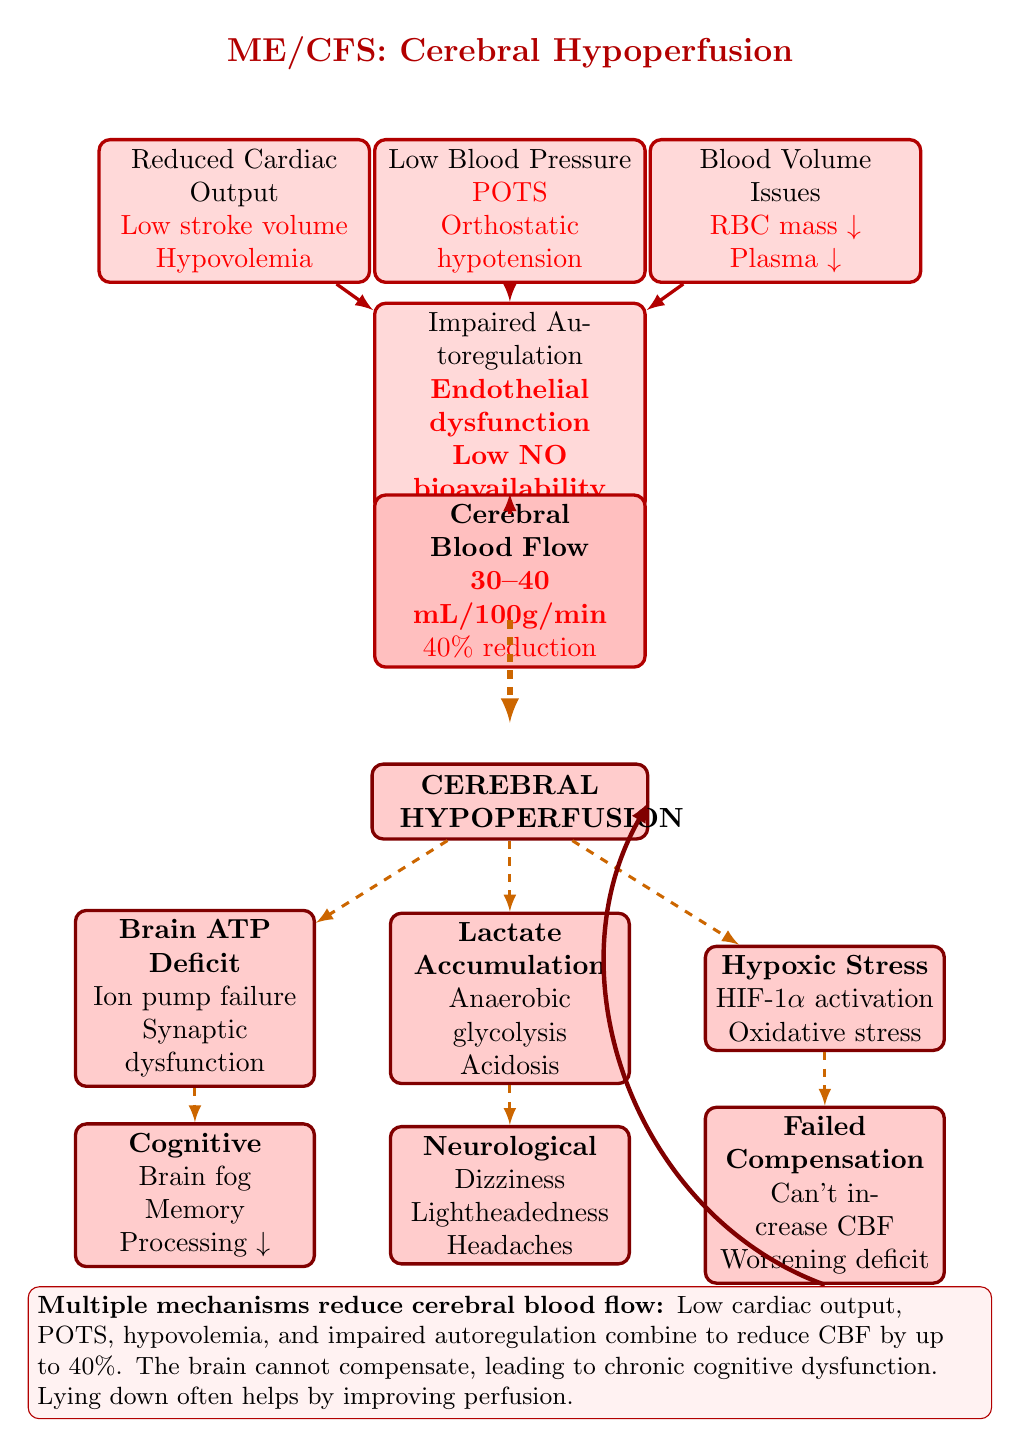
\begin{tikzpicture}[scale=1, every node/.style={scale=1},
    % Styles
    normal/.style={draw=green!70!black, fill=green!10, very thick, rounded corners, text width=3cm, align=center, minimum height=1cm},
    impaired/.style={draw=red!70!black, fill=red!15, very thick, rounded corners, text width=3.2cm, align=center, minimum height=1cm},
    severe/.style={draw=red!50!black, fill=red!25, ultra thick, rounded corners, text width=3.2cm, align=center, minimum height=1.1cm, drop shadow},
    pathological/.style={draw=red!50!black, fill=red!20, very thick, rounded corners, text width=2.8cm, align=center, minimum height=0.95cm},
    impaired-arrow/.style={-latex, very thick, red!70!black, line width=1.2pt},
    cascade-arrow/.style={-latex, thick, orange!80!black, dashed, line width=1.1pt},
    cycle-arrow/.style={-latex, ultra thick, red!50!black, line width=1.6pt},
    note/.style={font=\small\itshape, text width=2.4cm, align=left, red!60!black},
]

% Title
\node[font=\large\bfseries, red!70!black] at (0, 9) {ME/CFS: Cerebral Hypoperfusion};

% TOP: Impaired flow pathway
\begin{scope}[yshift=4.5cm]
    % Multiple contributors
    \node[impaired] (cardiac) at (-3.5, 2.5) {Reduced Cardiac\\Output\\{\color{red}Low stroke volume}\\{\color{red}Hypovolemia}};

    \node[impaired] (bp) at (0, 2.5) {Low Blood Pressure\\{\color{red}POTS}\\{\color{red}Orthostatic\\hypotension}};

    \node[impaired] (volume) at (3.5, 2.5) {Blood Volume\\Issues\\{\color{red}RBC mass $\downarrow$}\\{\color{red}Plasma $\downarrow$}};

    % Impaired autoregulation
    \node[impaired] (autoreg) at (0, 0) {Impaired Autoregulation\\{\color{red}\textbf{Endothelial dysfunction}}\\{\color{red}\textbf{Low NO bioavailability}}};
    \draw[impaired-arrow] (cardiac) -- (autoreg);
    \draw[impaired-arrow] (bp) -- (autoreg);
    \draw[impaired-arrow] (volume) -- (autoreg);

    % Reduced CBF
    \node[impaired, fill=red!25] (cbf) at (0, -2.2) {\textbf{Cerebral Blood Flow}\\{\color{red}\textbf{30--40 mL/100g/min}}\\{\color{red}40\% reduction}};
    \draw[impaired-arrow] (autoreg) -- (cbf);
\end{scope}

% BOTTOM: Cascade consequences
\begin{scope}[yshift=-3.5cm]
    % Central hypoperfusion
    \node[pathological, minimum width=3.5cm] (hypoperf) at (0, 3) {\textbf{CEREBRAL}\\  \textbf{HYPOPERFUSION}};

    % Three immediate consequences
    \node[pathological] (atp) at (-4, 0.5) {\textbf{Brain ATP}\\  \textbf{Deficit}\\Ion pump failure\\Synaptic dysfunction};

    \node[pathological] (lactate) at (0, 0.5) {\textbf{Lactate}\\  \textbf{Accumulation}\\Anaerobic glycolysis\\Acidosis};

    \node[pathological] (hypoxia) at (4, 0.5) {\textbf{Hypoxic Stress}\\HIF-1$\alpha$ activation\\Oxidative stress};

    \draw[cascade-arrow] (hypoperf) -- (atp);
    \draw[cascade-arrow] (hypoperf) -- (lactate);
    \draw[cascade-arrow] (hypoperf) -- (hypoxia);

    % Downstream symptoms
    \node[pathological] (cognitive) at (-4, -2) {\textbf{Cognitive}\\Brain fog\\Memory\\Processing $\downarrow$};

    \node[pathological] (neuro) at (0, -2) {\textbf{Neurological}\\Dizziness\\Lightheadedness\\Headaches};

    \node[pathological] (failed) at (4, -2) {\textbf{Failed}\\  \textbf{Compensation}\\Can't increase CBF\\Worsening deficit};

    \draw[cascade-arrow] (atp) -- (cognitive);
    \draw[cascade-arrow] (lactate) -- (neuro);
    \draw[cascade-arrow] (hypoxia) -- (failed);

    % Feedback loop
    \draw[cycle-arrow, bend left=50] (failed.south) to (hypoperf.east);
\end{scope}

% Arrow connecting top to bottom
\draw[cascade-arrow, line width=2pt] (0, 1.8) -- (0, 0.5);

% Key point box
\node[draw=red!70!black, fill=red!5, rounded corners, text width=12cm, align=left, font=\small] at (0, -7.5) {
\textbf{Multiple mechanisms reduce cerebral blood flow:} Low cardiac output, POTS, hypovolemia, and impaired autoregulation combine to reduce CBF by up to 40\%. The brain cannot compensate, leading to chronic cognitive dysfunction. Lying down often helps by improving perfusion.
};

\end{tikzpicture}
\caption{ME/CFS cerebral hypoperfusion cascade causing cognitive dysfunction.}
\label{fig:cerebral-hypoperfusion-mecfs}
\end{figure}
